\section{How a Viewpoint Cocoon Forms (RQ2)}
\label{sec:formation}

Ranking gives every user the same platform layer (\cref{sec:platform}). This section asks what personalisation adds for one user, the personal layer $V$ of \cref{eq:decomp}, for the case-study narrative: gender group labels within gender-and-marriage videos. We ask the question of three sources. The logs show what skew exists and with what it varies, but cannot say what caused it. Probing the recommender isolates its response to a controlled change in a user's history, but only for one step. The simulation chains such steps over months, at the price of a simplified user.

\subsection{In the logs: the personal layer}
\label{sec:logs}

\paragraph{The personal layer is wide, and topic share does not reveal it.} For the \nNHeavy{} users with at least 150 issue impressions, enough to estimate a personal share, we computed $V_u$ with empirical-Bayes shrinkage towards the platform share, equivalent to adding 12 issue videos at the platform share to each user's count. Its standard deviation is \nFunnelSD; \nFunnelHi\% of these heavy viewers meet the narrative at more than twice the platform odds, against \nFunnelLo\% at less than half, and the most skewed tenth average a share of \nTopDecileShare\% ($V=+\nTopDecileV$). \Cref{fig:logs}a plots $V_u$ against topic share. The spread widens as topic share grows, because a feed with more of the topic has more room to tilt, but its centre stays near zero: the correlation of $V_u$ with topic share is \nRhoMV, and with the category entropy of the feed, the quantity that cocoon checks report, $\nRhoEntV$. Category entropy tracks topic share closely ($\rho=\nRhoEntM$) and viewpoint skew hardly at all, as \cref{prop:topic} predicts.

\paragraph{Skew follows what the user recently finished.} If personalisation produces the personal layer, exposure should depend on the narrative's presence in the history that the recommender reads. We grouped issue impressions by the number of group-label videos among the user's previous 200 finished videos and computed, for each group, the log-odds of a group-label impression relative to the platform share (\cref{fig:logs}b). It rises steadily, from $\nObsZero$ for users with none to $+\nObsTop$ for users with more than twenty. This is an association, and users who finish many such videos may differ in other ways. The next experiment removes that doubt.

\begin{figure}[t]
  \centering
  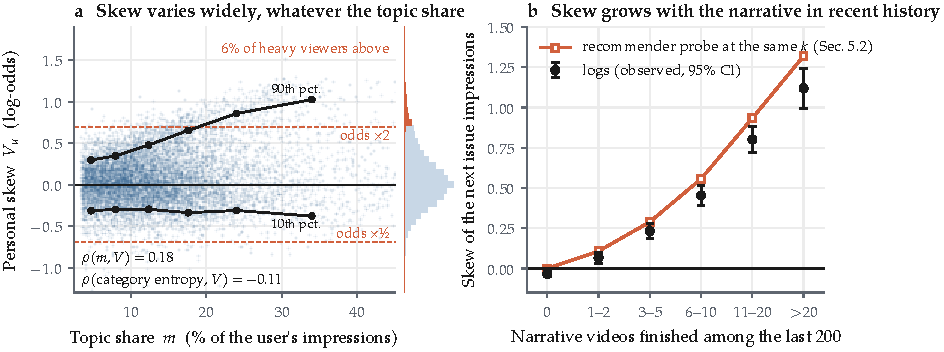
\includegraphics[width=\textwidth]{figures/fig_logs.pdf}
  \caption{Viewpoint skew in the logs. \textbf{(a)} Personal skew $V_u$ against topic share for \nNHeavy{} heavy viewers of the issue; lines show the 10th and 90th percentiles by topic share, and the histogram the marginal distribution of $V_u$. \textbf{(b)} Skew of the next issue impression by the number of group-label videos among the user's previous 200 finished videos (points, with 95\% intervals clustered by user), compared with the response of OneRec when the same number of videos is injected into a history (squares, from \cref{fig:probe}a).}
  \label{fig:logs}
\end{figure}

\subsection{Probing the recommender}
\label{sec:probe}

\paragraph{Protocol.} We took 200 users from OneRec's held-out split, each with their last 200 finished videos as history, and a fixed candidate set of 2{,}000 videos that appear in no history: 150 group-label videos, 350 other issue videos and 1{,}500 off-issue videos, sampled in proportion to exposure. For each user we computed the exact probability OneRec assigns to every candidate and read off two contrasts: the log-odds of issue against off-issue candidates (topic), and of group-label against other issue candidates (narrative). We then replaced $k$ randomly chosen off-issue videos in the history by $k$ held-out videos, either other issue videos (for the topic contrast) or group-label videos (for the narrative contrast), and recorded how the contrast changed. As a null, after injecting group-label videos we split the other-issue candidates at random into two halves and read the contrast between them, 200 times; with no real distinction it should stay near zero.

\paragraph{OneRec separates the narrative about two-thirds as sharply as the topic.} Ten issue videos added to a history raise the topic log-odds by $+\nProbeTopic$ (95\% CI \nProbeTopicLo--\nProbeTopicHi). Ten group-label videos raise the narrative log-odds by $+\nProbeNarr$ (\nProbeNarrLo--\nProbeNarrHi), in the same direction for \nProbeNarrPos\% of users, while ten other issue videos leave it at $\nProbeOther$ (\cref{fig:probe}a). The random-split null has standard deviation \nNullSD, so the narrative response is more than ten null standard deviations from zero. In the terms of \cref{prop:feedback}, the ratio of narrative to topic contrast is $c/t\approx\nProbeRatio$ at $k=10$, and 0.69 for the curves fitted across all five values of $k$. Both responses grow with $k$ and flatten, the narrative channel at about 1.5 and the topic channel near 2.8. The response at each $k$ lies close to the association seen in the logs (\cref{fig:logs}b), which the logs alone could not establish as causal.

\paragraph{``Not interested'' is read as interest.} OneRec's input has a separate field for videos the user marked ``not interested''. Placing the same ten group-label videos there does not push such videos down: the topic log-odds rise by $+\nNITopic$ and the narrative log-odds by $+\nNINarr$, about two-fifths of the response to finishing them, positive for \nNITopicPos\% and \nNINarrPos\% of users (\cref{fig:probe}b). The same videos in an extra field with a meaningless name produce almost the same response ($+\nFieldExtraTopic$ and $+\nFieldExtraNarr$). The model therefore treats any video mentioned in the history as a cue of interest, and the label on the field as a matter of degree. This is what a system trained to predict logged engagement would learn: people mark ``not interested'' on what their feed is full of. In the terms of \cref{prop:feedback}, the button has $\eta>0$.

\begin{figure}[t]
  \centering
  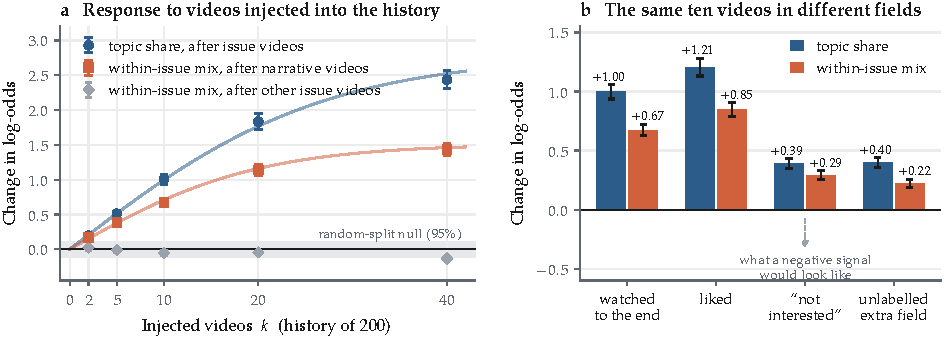
\includegraphics[width=\textwidth]{figures/fig_probe.pdf}
  \caption{Response of OneRec to controlled edits of 200 users' histories. \textbf{(a)} Change in the topic and narrative log-odds of the recommendations when $k$ videos are injected into the ``watched to the end'' field (means with 95\% intervals; curves are the saturating fit used by the simulation). \textbf{(b)} The same ten group-label videos placed in four different fields.}
  \label{fig:probe}
\end{figure}

\subsection{From one step to three months: a transparent simulation}
\label{sec:sim}

\paragraph{Model.} Probing gives the response to one edit. To follow a user over months we built a small simulator that instantiates \cref{eq:softmax}. Its recommender is fixed entirely by the probe; how users behave is a scenario, which we vary. Videos fall into four groups: group-label videos, other issue videos, rebuttals (1.5\% of issue impressions), and everything else. The recommender keeps an exponentially weighted profile of the user's last 200 finished videos and shifts the log-odds of the topic and of the narrative by the two fitted curves of \cref{fig:probe}a; with an empty profile it reproduces the platform shares of \cref{sec:platform}. A simulated user finishes an ordinary video with probability 0.38; a \emph{topic interest} $\varphi$ and a \emph{narrative preference} $\theta$ add to the log-odds of finishing issue videos and group-label videos respectively. We follow topic fans ($\varphi=0.8$) with strong ($\theta=2$, finishing 91\% of group-label videos against 58\% of other issue videos), mild ($\theta=1$), no, and negative preference, and a casual viewer ($\varphi=0$) with strong preference, each with 400 simulated users at 180 videos a day. \Cref{app:sim} lists all parameters, and \cref{tab:theta} gives the result for a full range of preferences.

\paragraph{Topic fans arrive at the same topic share and different views.} All four fans reach a topic share of 28--30\% within about six weeks (\cref{fig:formation}b). Their views diverge (\cref{fig:formation}a). After \nFormDays{} days the fan with strong preference has $V=+\nVStrong$: group-label videos are \nShareStrong\% of the issue videos in the feed, \nOddsStrong{} times the platform odds and \nTotalOddsStrong{} times supply. Half of this skew is in place after \nFormHalfDays{} days. The fan with mild preference settles at $+\nVMild$, the fan without preference at zero, and the fan who tends to skip the narrative at $\nVAverse$. The simulated fan with strong preference sits where the most skewed tenth of real heavy viewers do (\cref{sec:logs}).

\paragraph{A viewpoint cocoon needs volume.} The casual viewer has the same strong preference but little interest in the topic. Their topic share creeps from 2.4\% to \nMCasualOne\% and their skew stays at $+\nVCasual$: with four issue videos a day, too few group-label videos enter the history to move the narrative channel. This matches the funnel shape of \cref{fig:logs}a, and it means that the users most exposed to a viewpoint cocoon are the ones a topic-level check would flag only for their interest.

\paragraph{Formation hinges on what the recommender can separate.} \Cref{fig:formation}c varies the narrative response of the recommender while holding the topic response fixed. With no narrative contrast there is no skew, whatever the user prefers, as \cref{prop:feedback} states. At a ratio of 0.3, less than half the fitted one, the strong-preference fan reaches only $+\nSweepHalf$. Around the fitted ratio the curve is at its steepest, because exposure and consumption reinforce each other: more of the narrative shown means more of it finished. A recommender that separated narratives as well as it separates topics would take the same user to $+\nSweepOne$.

\begin{figure}[t]
  \centering
  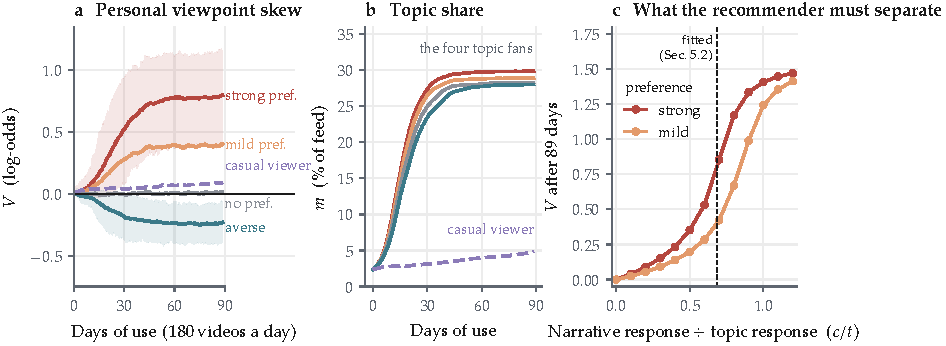
\includegraphics[width=\textwidth]{figures/fig_formation.pdf}
  \caption{Formation in the simulation fitted to \cref{fig:probe}a. \textbf{(a)} Personal skew over three months for five kinds of user (means of 400 simulated users; bands show the 10th to 90th percentile for two of them). \textbf{(b)} Topic share of the same users. \textbf{(c)} Skew after 89 days as a function of the recommender's narrative-to-topic response ratio; the dashed line marks the ratio fitted in \cref{sec:probe}.}
  \label{fig:formation}
\end{figure}
